\documentclass{beamer}

\usepackage[utf8]{inputenc}
\usepackage{default}

\usetheme{Warsaw}

\begin{document}

\begin{frame}{Motivation}

    \begin{figure}
    \centering
    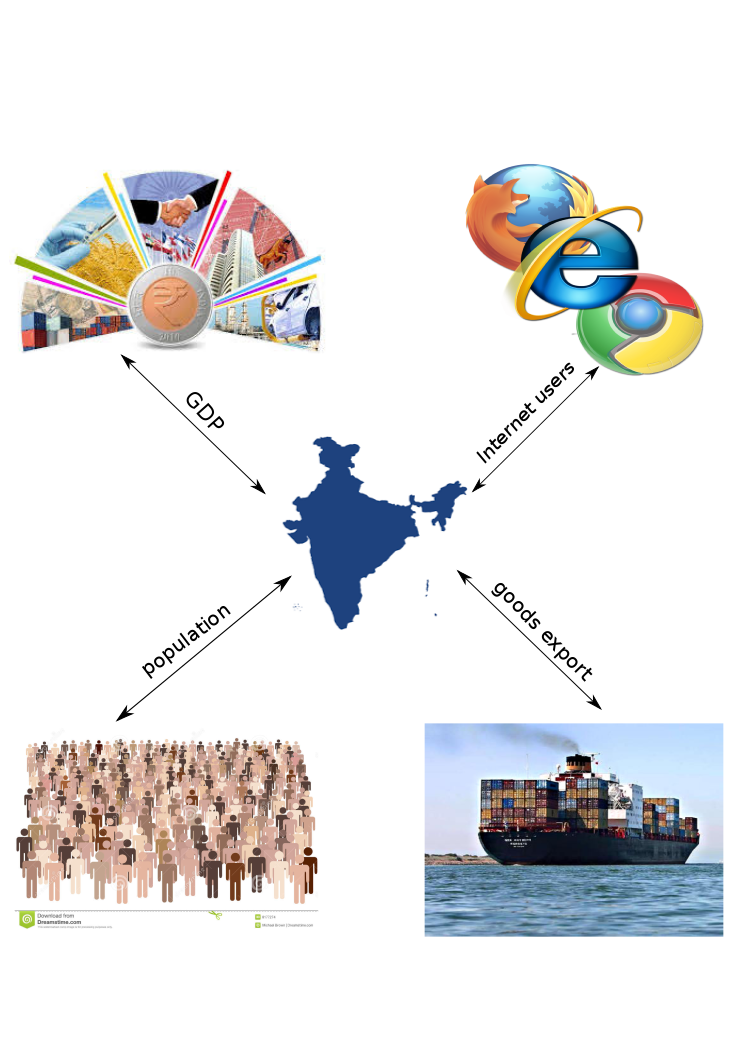
\includegraphics[width = 0.5\textwidth]{images/motivation}
  \end{figure}
 
\end{frame}


\begin{frame}{Motivation}
 
 \begin{itemize}
  \item Repositories of facts containing this information can be found at many places, like data.worldbank.org, Wikipedia infoboxes etc. \pause
  \item Countries are popular and finite, finding complete knowledge bases is possible. \pause
  \item What about less popular entities?  \pause
    \begin{itemize}
      \item What is the population of Arbit Apartments, Powai? \pause
      \item What is the GDP of Sugarcane Industry of India? \pause
      \item Percent of Internet users in Mumbai? 
    \end{itemize}
 \end{itemize} 
\end{frame}

\begin{frame}{Motivation}

\begin{itemize}
 \item  Good News!!! \pause
 \item  Web is huge, probably, there is some page which contains the information we are looking for. \pause
 \item The way in which you express a fact about an entity depends on the fact, and not the entity. \pause
 \item We may expect the sentence structure to be similar. \pause
 \begin{itemize}
    \item Population of India reached 1.3 billion, making it the second largest country in the world
    \item Population of Arbit Apartments, Powai reached 1300
 \end{itemize}
 
\end{itemize}
\end{frame}

\begin{frame}{Problem Statement}
 
 \begin{itemize}
  \item Given that we know a lot about countries, can we train extractors that run over the web and pull similar facts about other entities?
 \end{itemize}

 
\end{frame}




\end{document}
